\documentclass{article}

\usepackage{braket}
\usepackage{amsmath}
\usepackage{amsfonts}
\usepackage{amssymb}
\usepackage{xcolor}
\usepackage{chngcntr}
\usepackage{graphicx}
\usepackage{tikz}
\usepackage{pgfplots}
\usepackage{siunitx}
\usepackage{filecontents}
\usepackage{cite}
\usepackage{hyperref}
\usepackage{titlesec}
\pgfplotsset{width=15cm,compat=1.9}

\newcommand{\R}{\mathbb{R}}
\newcommand{\C}{\mathbb{C}}
\newcommand{\p}{\partial}
\renewcommand{\L}{\mathcal{L}}
\renewcommand{\H}{\mathcal{H}}

\long\def\/*#1*/{} %used to comment out multiple lines

\/*
     This text is commented out
*/

\counterwithin*{equation}{section}
\counterwithin*{equation}{subsection}

\setlength{\topmargin}{-.5in}
\setlength{\textheight}{9in}
\setlength{\oddsidemargin}{.125in}
\setlength{\textwidth}{6.25in}

\begin{document}
\begin{titlepage}
    \begin{center}
        \vspace*{2cm}
 
        \huge
        \textbf{ECE 434 Biophotonics Project}
     
        \vspace{1.5cm}
        \Large
        \textbf{Peter Grant, Evan Peters\\
        V00948581, V00954410}
 
        \vfill
             
        A Project Report on optical trapping\\
        For Dr. Tao Lu     

        \vspace{0.8cm}
      

             
        Department of Electrical and Computer Engineering\\
        University of Victoria\\
        April 8, 2024
             
    \end{center}
\end{titlepage}


\tableofcontents
\newpage

\addcontentsline{toc}{section}{Introduction}
\section*{Introduction}

Optical traps, often also called optical tweezers, are instruments that use the pressure exerted by intense laser light to manipulate particles in the micro and nanoscopic scale. The ability for lasers to trap and accelerate particles was first demonstrated by A. Ashkin in 1970 where two forces were identified: a scattering force in the direction of beam propagation, and a gradient force towards the center of the beam intensity \cite{PhysRevLett.24.156}. This gave rise to optical levitation, an arrangement in which the scattering force is used to suspend a particle against the force of gravity, and the gradient force to contain the particle in space. Ashkin refined this setup and reported a stable three dimensional optical trap in 1986, which used a convergent laser to trap a dielectric sphere at the point of convergence using laser gradient forces \cite{Ashkin:86}. This technology's ability to very precisely exert piconewtons of force uniformly on a particle, and at frequencies and power levels that do not cause radiation damage, has allowed for the widespread use of optical traps in microbiological research \cite{Bustamante2021}, \cite{Lang2003-ll}.

\addcontentsline{toc}{section}{Theory of Lasers}
\section*{Theory of Lasers}

To understand the theory of laser tweezers, it is necessary to understand the theory of lasers. This section will cover the basic theory of lasers, including the theory of light-matter interactions, how to use perturbation theory to determine transition rates, and the lasing principle.

\addcontentsline{toc}{subsection}{Light-Matter Interactions}
\subsection*{Light-Matter Interactions}

For an electron in an atom, the energy levels are quantized. As the electron changes energy levels, the energy is conserved, so an external particle must be involved. In the case of a laser, this particle is a photon \cite{Griffiths}. There are a couple important cases to consider for light-matter interactions. The first is the case of a two-level system, where the electron can only be in one of two states. Consider that the electron is in the lowest energy state, also known as the ground state. The system is depicted in the figure below. A photon is incident to the electron which has energy, or frequency, equal to the energy difference between the two states, or the resonant frequency. Then, the electron will gain energy and transition to the higher energy eigenstate \cite{Griffiths}.


\begin{figure}[h!]
    \begin{center}
    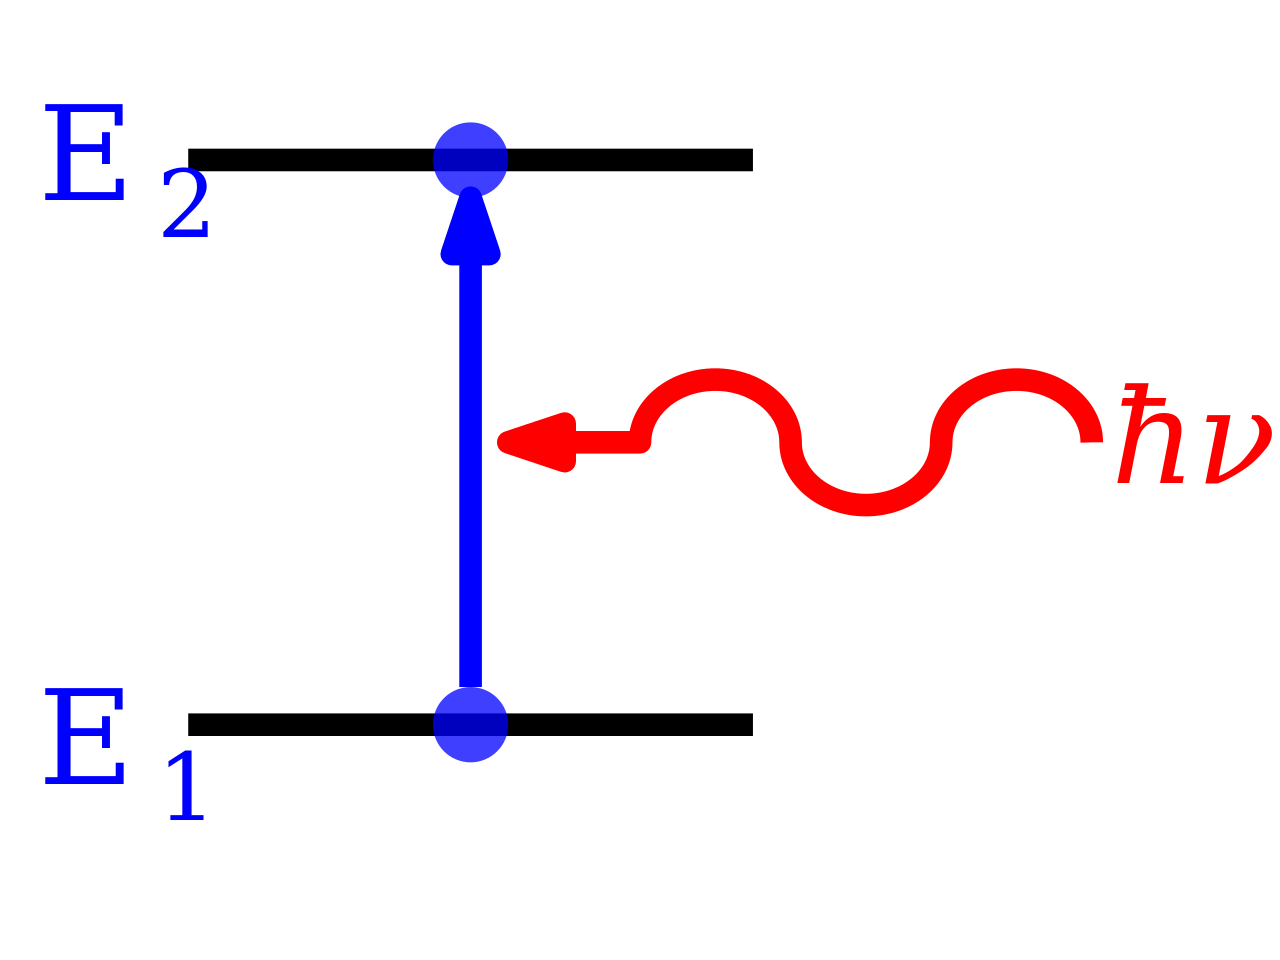
\includegraphics[width=0.5\linewidth]{Pictures/absorption.png}
    \caption{Absorption [wikipedia]}
    \label{fig:Absorption}
    \end{center}
\end{figure}


Consider the case where the electron is in the higher energy state. This higher energy state is not stable, and the electron will eventually transition back to the lower energy state. When this happens, a photon is emitted with energy equal to the energy difference between the two states. This is known as spontaneous emission, and is depicted in the figure below \cite{Griffiths}.

\begin{figure}[h!]
    \begin{center}
    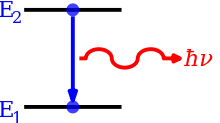
\includegraphics[width=0.5\linewidth]{Pictures/spontemission.png}
    \caption{Spontaneous Emission [wikipedia]}
    \label{fig:SpontEmission}
    \end{center}
\end{figure}


A similar event can occur where the electron is in the higher energy state, and a photon is incident with energy equal to the energy difference between the two states. In this case, the electron will lose energy and transition to the lower energy state. This is known as stimulated emission, and is depicted in the figure below \cite{Griffiths}.

\begin{figure}[h!]
    \begin{center}
    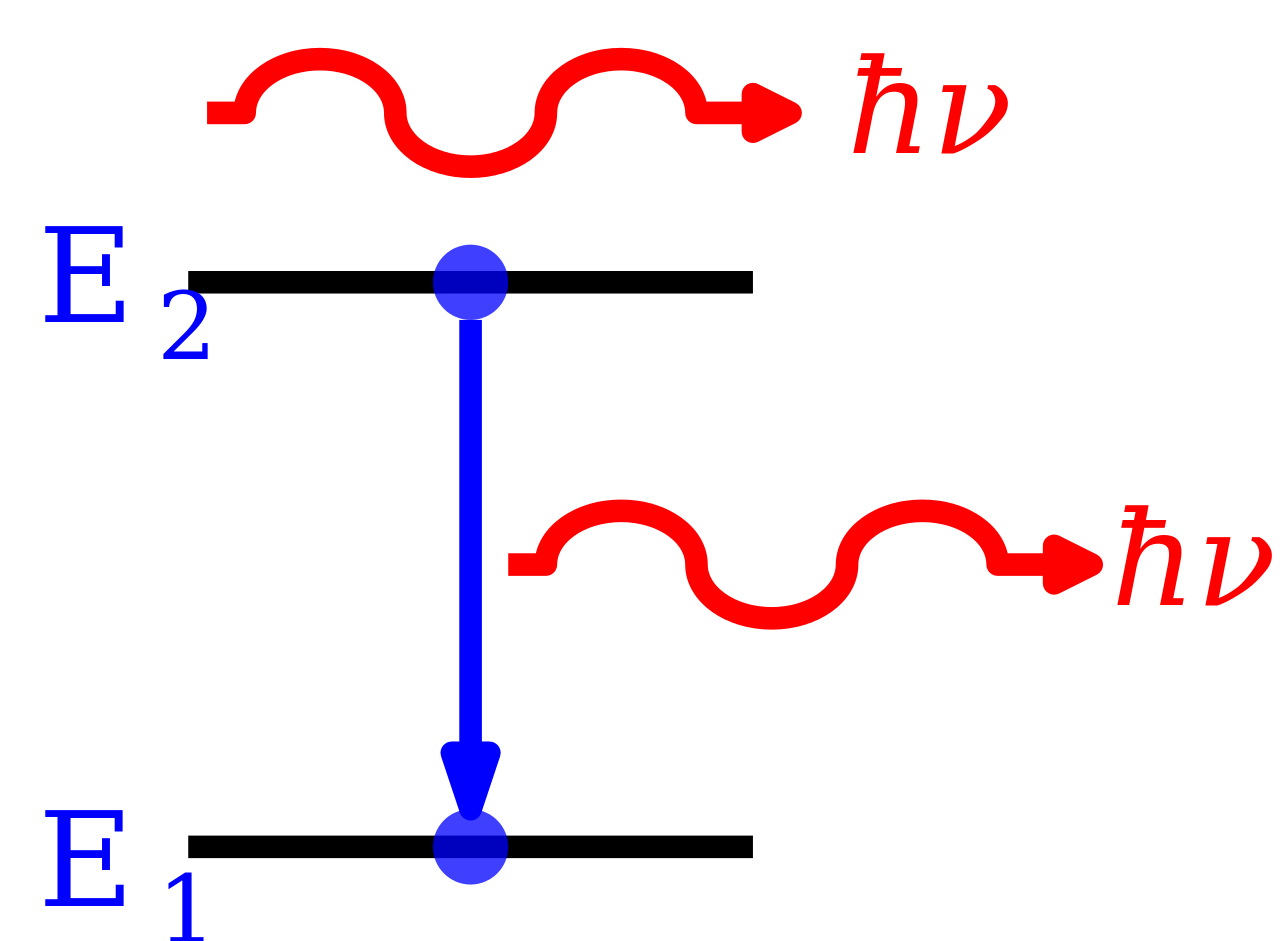
\includegraphics[width=0.5\linewidth]{Pictures/stimemission.png}
    \caption{Stimulated Emission [wikipedia]}
    \label{fig:Absorption}
    \end{center}
\end{figure}

Both forms of emission are similar, but come from different perturbations \cite{Griffiths}. So, it is clear that for a laser to work, the stimulated emission interaction must be the dominant interaction. How can this be achieved? To answer that, more theory is required.


\addcontentsline{toc}{subsection}{Perturbation Theory}
\subsection*{Perturbation Theory}


There are only a handful of potentials for which the Schr\"odinger equation can be solved exactly \cite{Griffiths}. For the vast majority of potentials, perturbation theory is necessary. The idea is to start with a simple potential for which the Schr\"odinger equation can be solved exactly, and then add a small perturbation to the potential. The Schr\"odinger equation can then be solved iteratively, with each term in the series representing a higher order correction to the wavefunction. 

In general, time-independent perturbation theory is used when the Hamiltonian can be written as the sum of two terms, $\H = \H^0 + \H'$, where $\H^0$ is the Hamiltonian for a system for which the Schr\"odinger equation can be solved exactly, and $\H'$ is a small perturbation \cite{Griffiths}.

For lasers, time-dependent perturbation theory is necessary. For example, the perturbation could be a sinusoidal electric field, which is used to model the interaction between light and matter. For time-dependent perturbation theory of a two-level system with two states that are eigenstates of the unperturbed Hamiltonian \cite{Griffiths},

\[ \hat{\H}^0\psi_a = E_a\psi_a,\quad \hat{\H}^0\psi_b = E_b\psi_b \]

The time evolution of the system is thus 
\[ \Psi(t) = c_a\psi_ae^{-iE_at/\hbar} + c_b\psi_be^{-iE_bt/\hbar} \]

Then, the perturbation is "turned on". The result is that the coefficients now depend on time 
\[ \Psi(t) = c_a(t)\psi_ae^{-iE_at/\hbar} + c_b(t)\psi_be^{-iE_bt/\hbar} \]

The desired quantities are $c_a(t)$ and $c_b(t)$. These can be found by solving the time-dependent Schr\"odinger equation with the perturbed Hamiltonian \cite{Griffiths}. 
\[ \hat{\H}\Psi = i\hbar\frac{\p\Psi}{\p t},\ \hat{\H} = \hat{\H}^0 + \hat{\H}'(t) \]

Solving this equation is not trivial, and is certainly beyond the scope of this paper. Please refer to the references for more information. However, because the states are orthogonal, the trick of taking the inner product of each state can be used. The essential result is \cite{Griffiths}
\begin{equation}
     \dot{c}_a = -\frac{i}{\hbar}\H'_{ab}e^{-i\omega_0t}c_b,\quad \dot{c}_b = -\frac{i}{\hbar}\H'_{ba}e^{i\omega_0t}c_a 
\end{equation}

Where 
\[ \omega_0 \equiv \frac{E_b - E_a}{\hbar} \]

So, this says that the probability of transitioning from state $a$ to state $b$ is proportional to the matrix element of the perturbation between the two states \cite{Griffiths}.

Thus far, the coefficients c are exact. However, to calculate them exactly requires infinitely higher order perturbations. Generally, the first order perturbation is sufficient, and will be examined for the rest of the paper.

\addcontentsline{toc}{subsection}{Sinusoidal Perturbations}
\subsection*{Sinusoidal Perturbations}

Since electromagnetic radiation is sinusoidal, it is extremely useful to look at sinusoidal perturbations. Consider the Hamiltonian
\[ \hat{\H}'(\vec{r},t) = V(\vec{r})\cos(\omega t) \]

This will have matrix element 
\[ \H'_{ab} = V_{ab}\cos(\omega t) \]

Where 
\[ V_{ab} = \braket{\psi_a|V(\vec{r})|\psi_b} \]

Plugging this result into (1) gives
\[ c_b(t) \approx -\frac{i}{\hbar}V_{ba}\int_0^tdt'\ \cos(\omega t')e^{i\omega_0t''}  \]
\[ = -\frac{V_{ba}}{2\hbar}\left[ \frac{e^{i(\omega_0+\omega)t}-1}{\omega_0+\omega} + \frac{e^{i(\omega_0+\omega)t}-1}{\omega_0-\omega} \right] \]

It is obvious that for frequencies far from the resonance frequency, the transition probability will be quite small. So, it is useful to only look at frequencies close to the resonant frequencies, and neglect the first term. This means that the transition probability for a sinusoidal perturbation is given by \cite{Griffiths} 
\[ P_{a\to b}(t) = |c_b(t)|^2 \approx \frac{|V_{ab}|^2}{\hbar}\frac{\sin^2\left[(\omega_0-\omega)t/2\right]}{(\omega_0-\omega)^2} \]

So, the incident electromagnetic wave will need to have a frequency close to the resonant frequency in order to have a significant transition probability \cite{Griffiths}.



\addcontentsline{toc}{subsection}{Lasing Principle}
\subsection*{Lasing Principle}

From the previous sections, it is clear that a laser will exploit the stimulated emission property to amplify light. It is also clear that stimulated emission produces photons at the resonant frequency. However, consider a material made up of many electrons in a two-level system. The electrons will be in a Boltzmann distribution of energy levels, and so the electrons will not all be in the higher energy state. This means that absorption will be the most common interaction, and there will be no light amplification through stimulated emission of radiation \cite{Griffiths}. 

Thus, it is necessary to have more electrons in the excited state than the ground state. This is known as a population inversion, and requires external energy. To achieve higher gain, the material is placed between two mirrors to form a Fabry-Perot cavity. One of the mirrors is partially transparent to allow the light to escape.

The result of a laser is extremely coherent light that can be focused to a small spot. This is ideal for optical trapping, and is the basis for the theory of laser tweezers.


\addcontentsline{toc}{section}{Theory of Laser Tweezers}
\section*{Theory of Laser Tweezers}

Now that the theory of lasers has been covered, the theory of laser tweezers can be discussed. This section will cover the theory of laser tweezers, including some of the various models.

\addcontentsline{toc}{subsection}{The Ray Optics Model}
\subsection*{The Ray Optics Model}

The simplest explanation of how optical traps work is the ray optics model. This model treats the trapped particle as a dielectric sphere, and the laser as a Gaussian beam \cite{UToronto}. As the light get refracted through the object being trapped, there will be a change in the momentum of every photon. This change in momentum will result in a force on the object. The force is given by \cite{UToronto}

\[ \vec{p} = \hbar \vec{k} \]
\[ \vec{F} = \frac{\p \vec{p}}{\p t} \]

So, the force on the object is given by the gradient of the intensity of the laser beam, and moves the object to the most intense point of the laser \cite{UToronto}. The particle will experience a restoring force governed by Hooke's law \cite{UToronto}.

\begin{figure}[h!]
    \begin{center}
    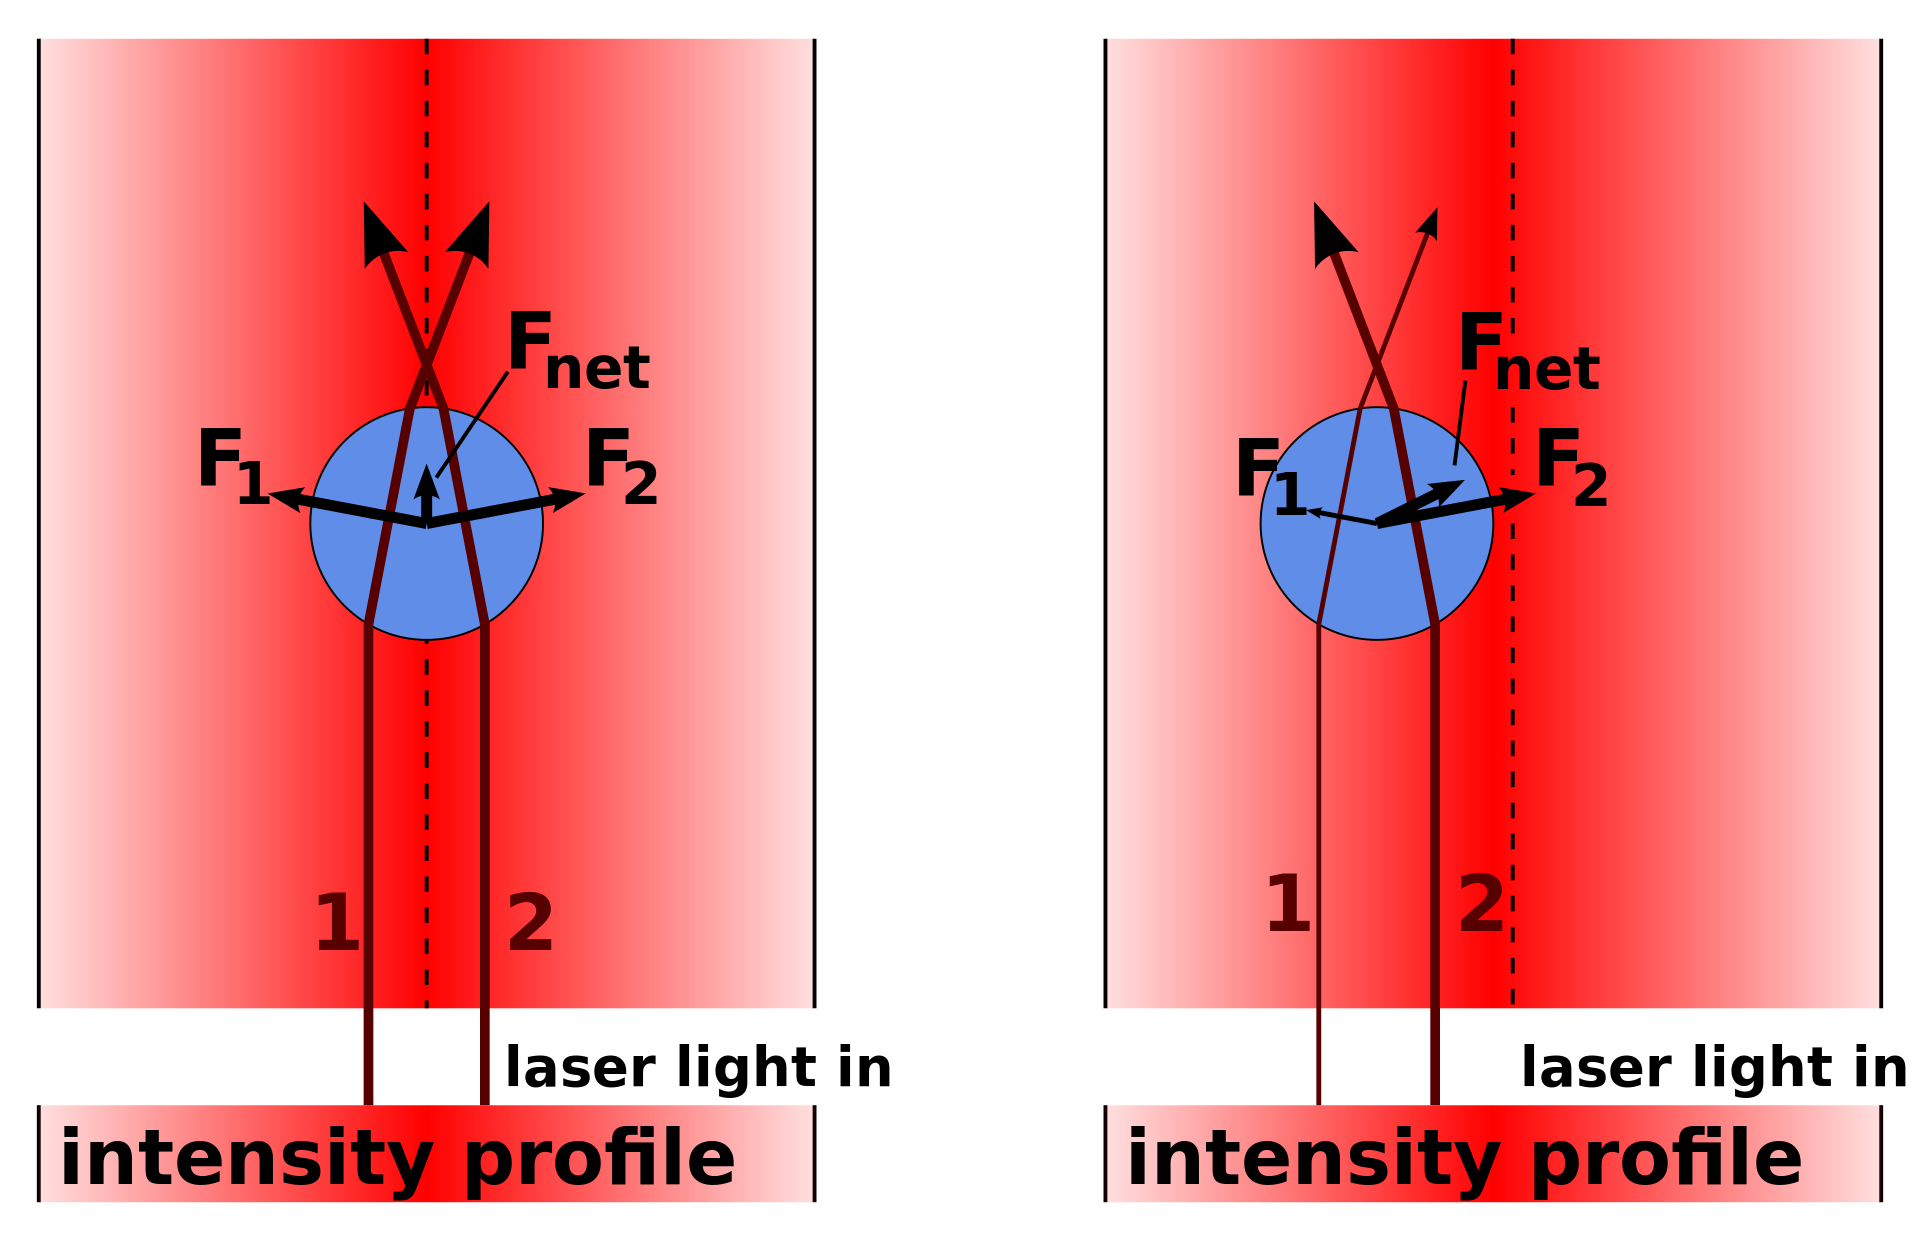
\includegraphics[width=0.5\linewidth]{Pictures/Optical_trap_unfocused.png}
    \caption{Optical Trapping Principle with Unfocused Laser [wikipedia]}
    \label{fig:unfocused}
    \end{center}
\end{figure}

However, there is no force preventing the object from moving in the direction of the laser, so the solution is to focus the light.

\begin{figure}[h!]
    \begin{center}
    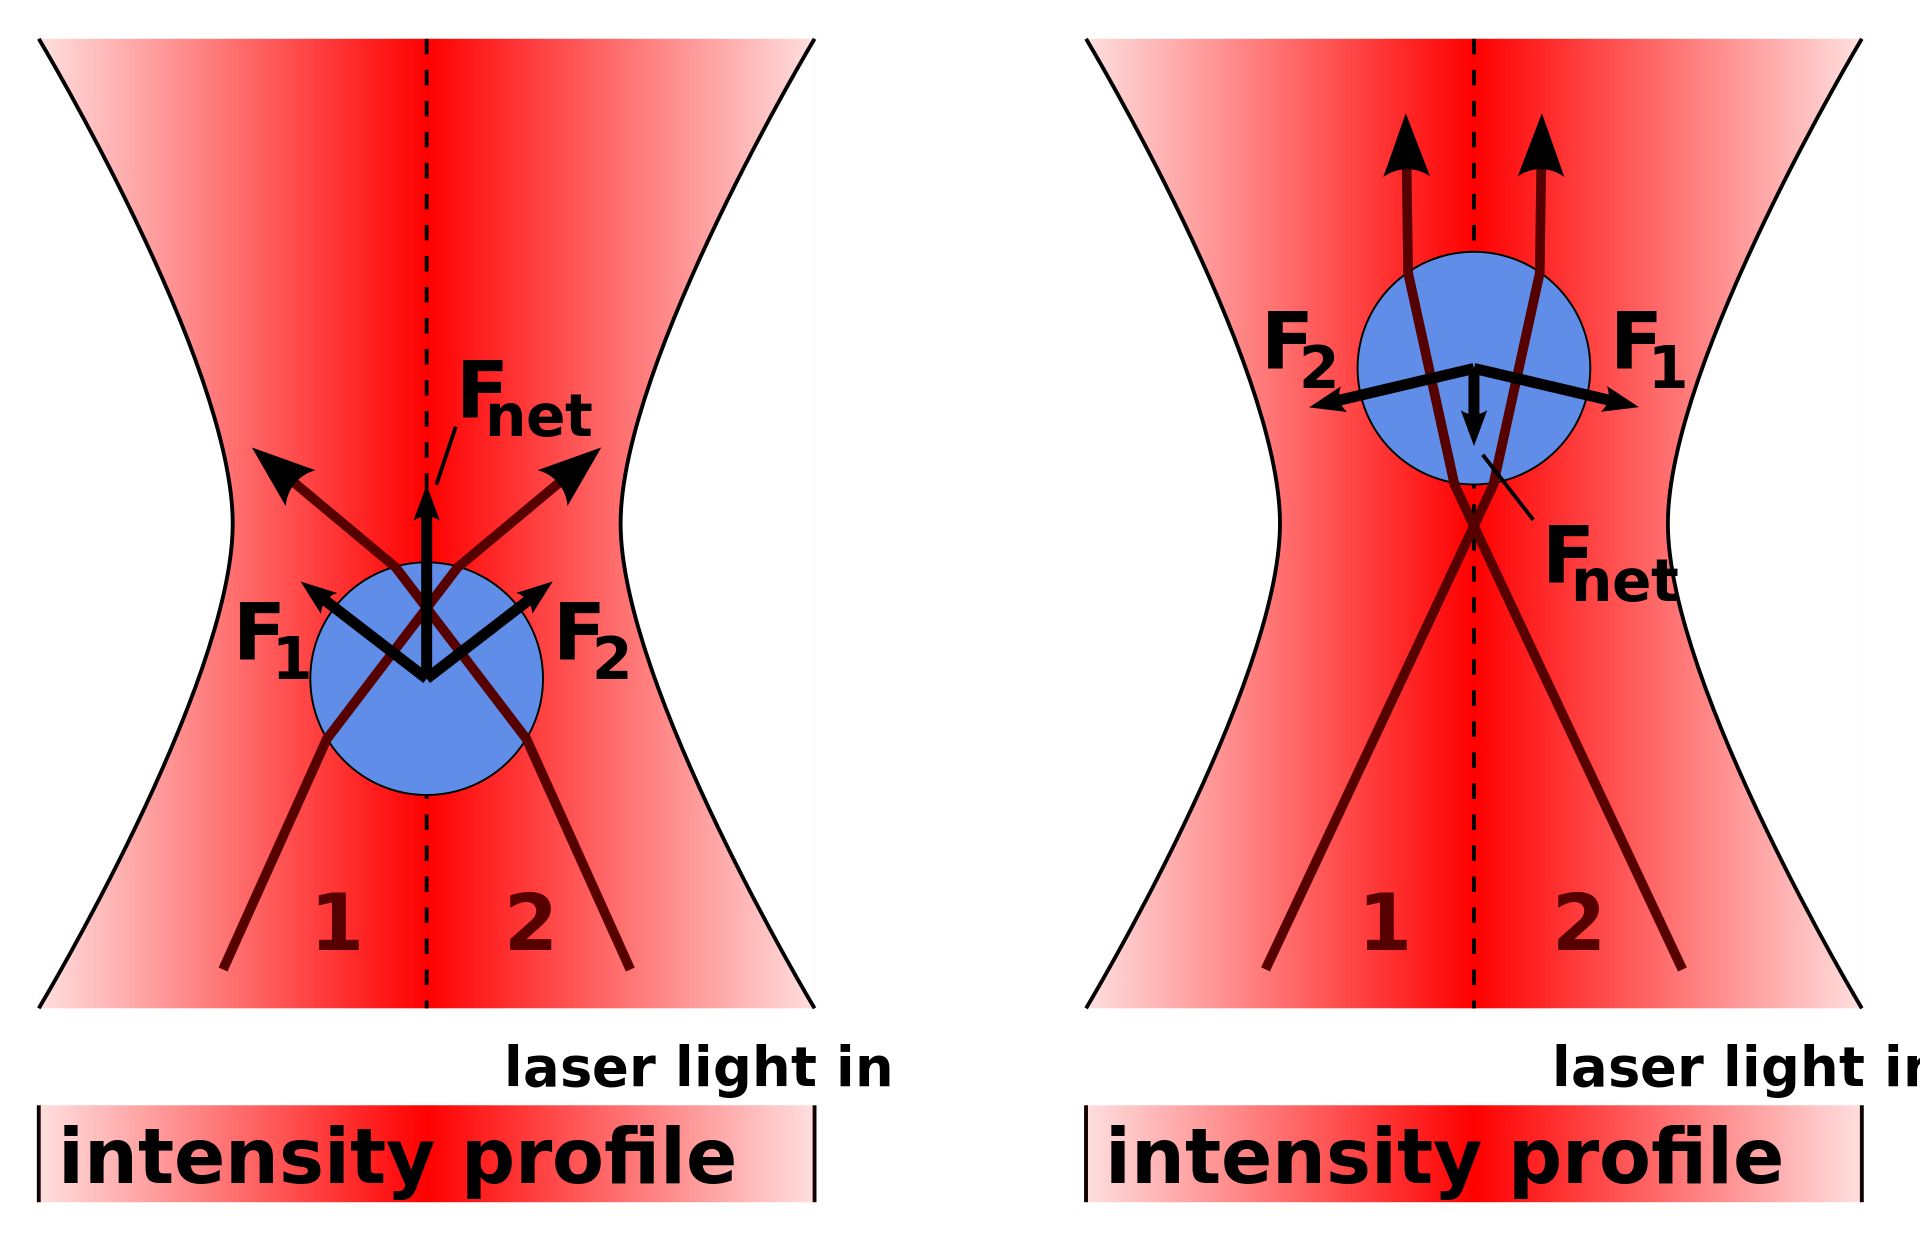
\includegraphics[width=0.5\linewidth]{Pictures/Optical_trap_focused.png}
    \caption{Optical Trapping Principle with focused Laser [wikipedia]}
    \label{fig:focused}
    \end{center}
\end{figure}
\newpage
From the figure, this will keep the object directly at the focal point of the laser.


\addcontentsline{toc}{subsection}{The Electric Dipole Model}
\subsection*{The Electric Dipole Model}

For small objects, the ray optics model no longer works. So, more theory is required. The object can be modeled as an electrical dipole to approximate the photon and particle interactions. The force acting on a single point charge placed in a magnetic field is known as the Lorentz force \cite{UToronto}

\[ \mathbf{F} = (\mathbf{p}\ \cdot\mathbf{\nabla})\mathbf{E} + \frac{d\mathbf{p}}{dt}\times\mathbf{B} \]

Here, $\mathbf{p}$ is the dipole moment of the object, $\mathbf{E}$ is the electric field, and $\mathbf{B}$ is the magnetic field. The first term is the force due to the electric field, and the second term is the force due to the magnetic field.

Through the use of polarizability, $\alpha$, the dipole can be eliminated.

\[ \mathbf{F} = \alpha\left[ (\mathbf{E}\cdot\mathbf{\nabla})\mathbf{E} + \frac{d\mathbf{E}}{dt}\times\mathbf{B} \right]  \]
\[ \mathbf{F} = \alpha\left[ \frac{1}{2}\mathbf{\nabla}\mathbf{E}^2 + \frac{d}{dt}(\mathbf{E}\times\mathbf{B}) \right]  \]

Then, the term on the right is the time derivative of the Poynting vector. For a CW laser, this term is simply zero
\[ \mathbf{F} = \frac{1}{2}\alpha\nabla E^2 \]

Again, the force depends on the gradient of the intensity of the laser beam. This is the same result as the ray optics model, but with a more rigorous derivation \cite{UToronto}.


\addcontentsline{toc}{section}{Applications}
\section*{Applications}

While the precision of optical traps makes them suitable for nearly any application involving the manipulation of micro and nanoparticles, they have seen the most use by far while facilitating novel research in the field of microbiology. This includes the manipulation of entire cells down to that of single molecules, and has resulted in significant findings on essential mechanisms like DNA transcription and molecular motor mechanics \cite{Bustamante2021}, \cite{2018_Polimeno}. It is worth noting that other technologies, such as atomic force microscopy and magnetic tweezers have been used in the same applications as optical traps, each with their benefits and drawbacks. Notably, atomic force microscopy often affords higher (>100pN) forces and magnetic tweezers offer advantages at lower (<1pN) forces; However, atomic force microscopy's limited force resolution and magnetic tweezer's limited spatial resolution still makes optical traps the most popular choice in biophysical research \cite{Bustamante2021}. Optical traps have been available as a technology for nearly 40 years and have been applied to many different fields of research; the following sections describe some particularly impactful examples of optical trap applications.


\addcontentsline{toc}{subsection}{Single-Cellular Manipulations}
\subsection*{Single-Cellular Manipulations}

While being developed, optical traps were originally used on silica dielectric beads since their uniformly round shape and transparency made the trapping effect more pronounced. Fortunately, many cells exhibit similar properties and as such were natural subjects for laser tweezer manipulation. As early as 1987 Ashkin et al. reported using IR laser traps to observe Escheria Coli and yeast reproduction, as well as the manipulation of red blood cells, spirogyra (algae), and protozoa (unicellular eukaryotes) \cite{Ashkin1987}. All of this was performed reportedly damage free, and on a variety of bodies which were still trapped by the gradient forces of the laser despite their nonspherical, nonuniform shapes. These observations clearly demonstrated the utility of optical traps in microbiological research, and resulted in a wide range of studies involving optical traps, often analysing cell replication, motility, and morphology \cite{Lang2003-ll}, \cite{Mammen1996-qn}, \cite{Svoboda1992-xm}, \cite{DAI1995988}. Optical traps have also seen extensive use alongside other methodologies such as microsurgery, optical scissors, and fluorescence characterization to allow for new research approaches \cite{Lang2003-ll}, \cite{LIANG1993110}.



\addcontentsline{toc}{subsubsection}{Red Blood Cell Mechanical Characteristics}
\subsubsection*{Red Blood Cell Mechanical Characteristics}

Optical tweezers have seen considerable use characterising the mechanical properties of red blood cells, either through directly trapping the cells or by manipulating trapped beads that are then attached to the cells \cite{2018_Polimeno}, \cite{Henon1999-nc}. Manipulation of these bead “handles” using a ND:YAG allowed Hénon et Al. to stretch the cells as shown in figure 1. Measurements of this deformation allowed for exact modelling of the elastic and shearing characteristics of the cells. Abnormalities in these mechanical characteristics of red blood cells have been linked to several pathological conditions, and red blood cell testing with optical traps has yielded results towards diagnosing and treating malaria, diabetic retinopathy, and birdshot chorioretinopathy \cite{2018_Polimeno}.

\begin{figure}[h!]
    \begin{center}
    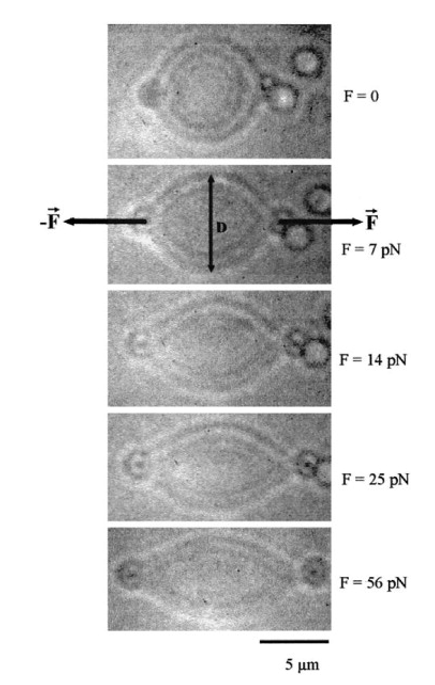
\includegraphics[width=0.5\linewidth]{Pictures/rbc.png}
    \caption{Discotic Red Blood Cell being Deformed by Two Optically Trapped Beads}
    \label{fig:rbc}
    \end{center}
\end{figure}
\newpage

\addcontentsline{toc}{subsubsection}{Gamete Manipulation}
\subsubsection*{Gamete Manipulation}

One notable area of full-cell manipulation research is the manipulation of gamete cells for fertilisation and force generation measurements. In 1996 Clement-Sengewald et Al. demonstrated the utility of optical trapping in contactless artificial fertilisation by first drilling a hole in the zona of bovine oocytes using a nitrogen laser, then manipulating sperm into the oocyte using a ND:YAG optical trap \cite{Clement-Sengewald1996-lc}, \cite{Antinori1996-dt}. This approach significantly increased the successful fertilisation rate even with very weak sperm, with its precise and entirely contactless nature showing advantages over traditional needle and pipette micromanipulation techniques.


\addcontentsline{toc}{subsection}{Organelle \& Subcellular Manipulations}
\subsection*{Organelle \& Subcellular Manipulations}

The most popular area of research involving optical traps is the manipulation and investigation of subcellular components. Since the traps are highly precise and mainly non-destructive, they are well suited to manipulating components even down to a unimolecular level \cite{Bustamante2021}, \cite{2018_Polimeno}. These unique traits have allowed for highly impactful research to be performed analysing fundamental biological mechanisms in unprecedented detail. Some of the most notable examples of this include the investigations performed on the structure of nucleic acids, and the mechanisms behind essential enzymes and proteins like RNA Polymerase and Kinesin.



\addcontentsline{toc}{subsubsection}{DNA Structure \& Interactions}
\subsubsection*{DNA Structure \& Interactions}

DNA's mechanical properties regulate many of its interactions with proteins, and measuring and understanding these characteristics is an important step in understanding essential cellular processes \cite{Bustamante2021}. Additionally, manipulation of DNA offers a means to control the important processes it is involved in, such as RNA transcription or protein folding. In order to accurately control these processes, extensive research has been performed characterising the elastic parameters of DNA with the aid of dielectric trapped beads to which the DNA is anchored \cite{Lang2003-ll}. Using these measurements, new configurations investigating DNA-Protein interactions have been investigated, with primary configurations being stretching, unzipping, twisting, and fluorescence manipulation as shown in the figure below.

\begin{figure}[h!]
    \begin{center}
    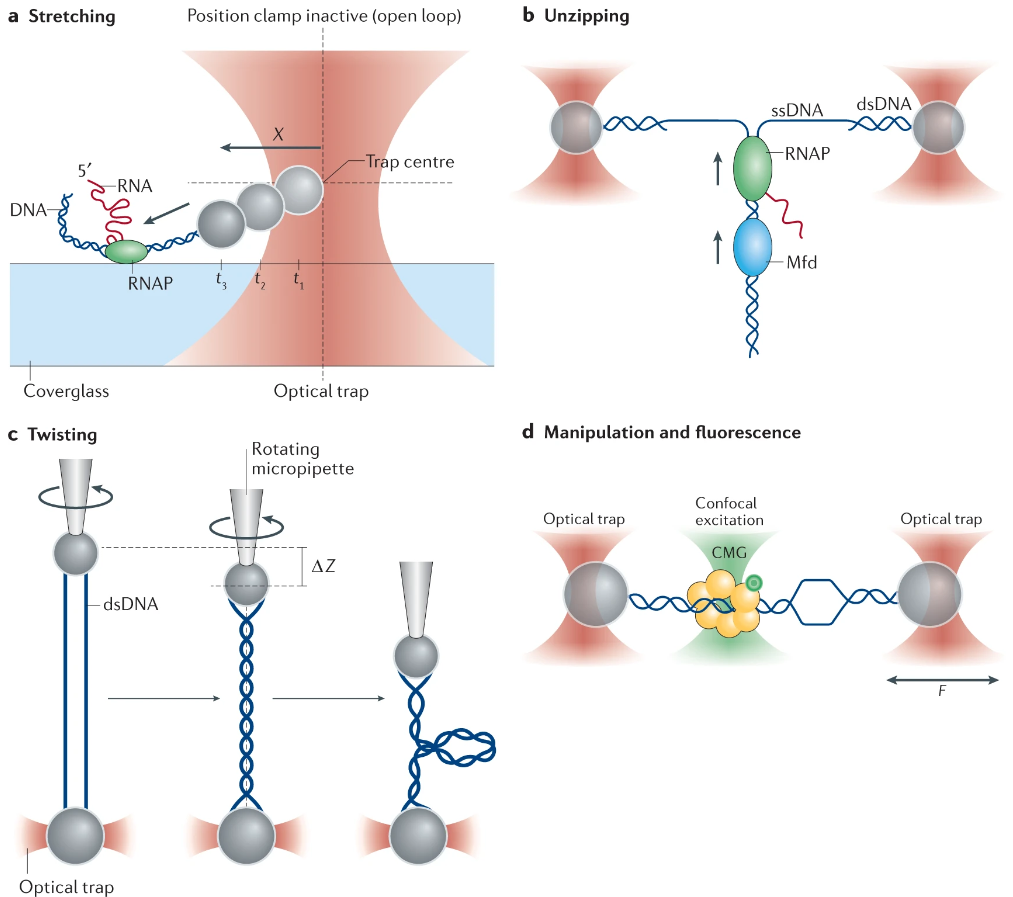
\includegraphics[width=0.5\linewidth]{Pictures/applications.png}
    \caption{Example Applications Studying Protein-DNA Interactions}
    \label{fig:app}
    \end{center}
\end{figure}
\newpage

Stretching, shown in Figure 7a, involves anchoring DNA to a trapped bead and anchoring a motor protein - in this case RNA Polymerase (RNAP) - to a surface or another bead. The motor protein's process is measured as the stretched DNA pulls the trapped bead out of the trap, with applied trap loads being able to stall the protein's precession entirely, and advanced setups being able to detect movement at base-pair resolution (~3.7Å) \cite{Abbondanzieri2005}, \cite{science.1235441}. This method has given insight into how RNAP displaces DNA bound proteins, such as histones, as well as how DNA encoded information regulates RNAP behaviour and transcription \cite{Abbondanzieri2005}. Similarly, unzipping as shown in Figure 2b divides the double strand DNA (dsDNA) into single strands (ssDNA) held separately as the RNAP processes down the stand. This is used to measure the base-pair bond strength for various sequences, and can also be used to measure procession rate similar to stretching \cite{Bustamante2021}. Twisting is the less common configuration shown in Figure 2c, and is primarily used to measure DNA elastic properties as described above. Twisting has also been used to measure DNA-protein interactions under stress, allowing investigations into how RNAP functions on constantly coiling DNA strands \cite{science.1235441}. Lastly, Figure 2d shows optical trap manipulation paired with fluorescence, which is used to better indicate the location of molecules of interest. Regions could be molecules, proteins, or sections of DNA fluoresced using conventional methods, and stabilising the regions with optical traps has allowed for more effective imaging and analysis \cite{Harada1999-bb}.




\addcontentsline{toc}{subsubsection}{Molecular Motor Mechanochemistry}
\subsubsection*{Molecular Motor Mechanochemistry}

Molecular motors are nanometre-scale proteins that generate force from local energy for many essential cellular functions. RNA Polymerase is one such motor protein discussed in the previous section under the context of DNA interaction, however optical traps have been used extensively to characterise other important motor proteins \cite{Bustamante2021}, \cite{Lang2003-ll}. Kinesin, a protein which hydrolyzes ATP to transport vesicles along microtubules, has been extensively investigated using this technology. By attaching a trapped bead to one end of the kinesin force applied to the bead can place the protein on a microtubule, and allow it to process or stall it similar to during stretching with RNAP \cite{Block1990}. Experiments of this nature have identified that Kinesin steps in 8nm increments, that each step requires one ATP, and that the kinesin detaches from the microtubule for a brief period with each step \cite{Lang2003-ll}, \cite{Block1990}. Stress testing motor proteins like kinesin is an ideal application for optical traps that can easily contest, counteract, and measure the force exerted by these proteins, resulting in a clearer understanding of how these essential proteins function.



\addcontentsline{toc}{section}{Conclusions}
\section*{Conclusions}

Optical tweezers have been a revolutionary technology in the field of biophotonics, allowing for the manipulation of particles at the micro and nanoscopic scale with unprecedented precision. The technology has been used in a wide range of applications, from the manipulation of entire cells to the study of single molecules. Optical tweezers will be an incredibly useful tool in the future of biophotonics, and will continue to be used at the frontiers of research.

\newpage
\bibliography{Term_Paper}
\bibliographystyle{ieeetr}



\end{document}